%Fiquemos com Deus e Nossa Senhora!
%Sao Jose de Cupertino rogai por nos!!
% ### Uses XeLaTeX ### %
% ### Needs beamer-master ### %
\documentclass[aspectratio=169]{beamer} %. Aspect Ratio 16:9

\usetheme{AI2} % beamerthemeSprace.sty
\usepackage[portuguese]{babel}
\usepackage[utf8]{inputenc}
\usepackage[T1]{fontenc}
\usepackage{ragged2e,graphicx,gensymb,bm,epsfig}

\DeclareMathOperator*{\argmin}{arg\,min}
\DeclareMathOperator*{\argmax}{arg\,max}

% DATA FOR FOOTER
\date{2021}
\title{- Redes Neurais Convolucionais}
\author{João Paulo Papa}
\institute{Advanced Institute for Artificial Intelligence (AI2)}

\begin{document}
% ####################################
% FIRST SLIDE 						:: \SliTit{This is the Title of the Talk}{A. B. Name}{Sprace}
% SUB-TITLE SLIDE 					:: \SliSubTit{<title>}{<explanation}
% SUB-SUB-TITLE SLIDE				:: \SliSubSubTit{<title>}{<explanation}
% SLIDE WITH TITLE 					:: \SliT{Title}{Content}
% SLIDE NO TITLE 						:: \Sli{Content} 
% SLIDE DOUBLE COLUMN WITH TITLE 	:: \SliDT{Title}{First Column}{Second Column}
% SLIDE DOUBLE COLUMN NO TITLE 		:: \SliD{First Column}{Second Column}
% SLIDE ADVANCED WITH TITLE 			:: \SliAdvT{Title}{Content}
% SLIDE ADVANCED NO TITLE 			:: \SliAdv{Content}
% SLIDE ADVANCED DOUBLE WITH TITLE 	:: \SliAdvDT{Title}{First Column}{Second Column}
% SLIDE ADVANCED DOUBLE NO TITLE 	:: \SliAdvD{First Column}{Second Column}
% SLIDE BLACK						:: \Black{ <Content> }
% SLIDE WHITE						:: \White{ <Content> }
% ITEMIZATION 						:: \begin{itemize}  \iOn{First} \iTw {Second} \iTh{Third} \end{itemize}
% COMMENT TEXT				 		:: \note{<comment>}
% SECTION 							:: \secx{Section} | \secxx{Sub-Section}
% BOLD SPRACE COLOR				:: \bfs{<text>}
% TABLE OF CONTENT					:: \tocitem{<title>}{<content>}
% LEFT ALIGN EQUATION				:: \begin{flalign*}  & <equation> &   \end{flalign*}
% CENTER ALIGN EQUATION	S			:: \begin{gather*} <equations>  \end{gather*}
% SLASH								:: \slashed{<>}
% BAR								:: \barr{<letter>} instead of \bar{<letter>}
% THEREFORE						:: use \portanto (larger and bold}
% 2 or 3 MATH SYMBOLS				:: \overset{<up>}{<down>} &  \underset{<below>}{\overset{<above>}{<middle>}}  
% INSERT TEXT IN FORMULA			:: \ins{<text>}
% EXERCISE							:: \exe{<exercise #>}{<exercise text>}
% SUGGESTED READING BOX			:: \sug{<references>}
% CITATION							:: \cittex{<citation>}
% CITATION DOUBLE COLUMN 			:: \cittexD{<citation>}
% TEXT POSITION						:: \texpos{<Xcm>}{<Ycm>}{<text>} origin = center of slide : x right | y down
% REFERENCE AT BOTTOM  S/D SLIDE		:: \refbotS{<reference>} \refbotD{<reference>}
% HIDDEN SLIDE						:: \hid
% COLOR BOX 						:: \blu{blue} + \red{rec} + \yel{yellow} + \gre{green} + \bege{beige}
% FRAME 							:: \fra{sprace} \frab{blue} \frar{red} + \fray{yellow} + \frag{green}		
% FIGURE 							:: \img{X}{Y}{<scale>}{Figure.png} 
% FIGURE							:: \includegraphics[scale=<scale>]{Figures/.png}
% FIGURE DOUBLE SLIDE NO TITLE		::  \img{-4}{0.5}{<scale>}{Figure.png} % Image 1st half
%									::  \img{4}{0.5}{<scale>}{Figure.png} % Image 2nd half
% FIGURE DOUBLE SLIDE WITH TITLE		::  \img{-4}{0}{<scale>}{Figure.png} % Image 1st half
%									::  \img{4}{0}{<scale>}{Figure.png} % Image 2nd half
% INCLUDING SWF (Flash)				:: \usepackage{media9} and \includemedia >> USE ACROBAT <<
%%%%%%%%%%%%%%%%%%%%%%%%%%%%%%%%%%%%%%%%%%%%%%%%%%
% ###############################################################################
% FIRST SLIDE
\SliTit{{\LARGE Redes Neurais Convolucionais}}{Advanced Institute for Artificial Intelligence -- AI2}{https://advancedinstitute.ai}
%%%%%%%%%%%%%%%%%%%%%%%%%%%%%%%%%%%%%%%%%%%%%%%%%%
% ###############################################################################
% SLIDE SUB-TITLE
%\SliSubTit{Sub-Title}{Description}{}
%%%%%%%%%%%%%%%%%%%%%%%%%%%%%%%%%%%%%%%%%%%%%%%%%%
% ###############################################################################
%\SliSubSubTit{Sub-Sub-Title}{Description}
 %%%%%%%%%%%%%%%%%%%%%%%%%%%%%%%%%%%%%%%%%%%%%%%%%%


\SliT{Introdução}{

\justifying Técnicas de \textbf{aprendizado em profundidade}, do inglês \emph{deep learning}, pertencem a um ramo da área de aprendizado de máquina e que fazem uso de redes neurais com diversas camadas. A ideia é, basicamente, empregar camadas para aprender, progressivamente, diferentes níveis de características a partir de um dado de entrada. Os níveis de abstração vão aumentando à medida que mais camadas são utilizadas para extração e aprendizado das características.\newline

\justifying Dentre as técnicas de aprendizado em profundidade, uma atenção especial tem sido dada às Redes Neurais Convolucionais, do inglês \emph{Convolutional Neural Networks} - CNNs. Tais modelos possuem uma alta capacidade de representação dos dados, com resultados promissores em inúmeras áreas do conhecimento.
}

\Sli{
\justifying A ideia consiste, basicamente, em utilizar "dados crus"\ (\emph{raw data}) como entrada e permitir com que a rede aprenda as características que são mais importantes para o problema em questão. Desta forma, eliminamos a necessidade de extrair características de maneira manual (\emph{handcrafted features}).

\begin{center}
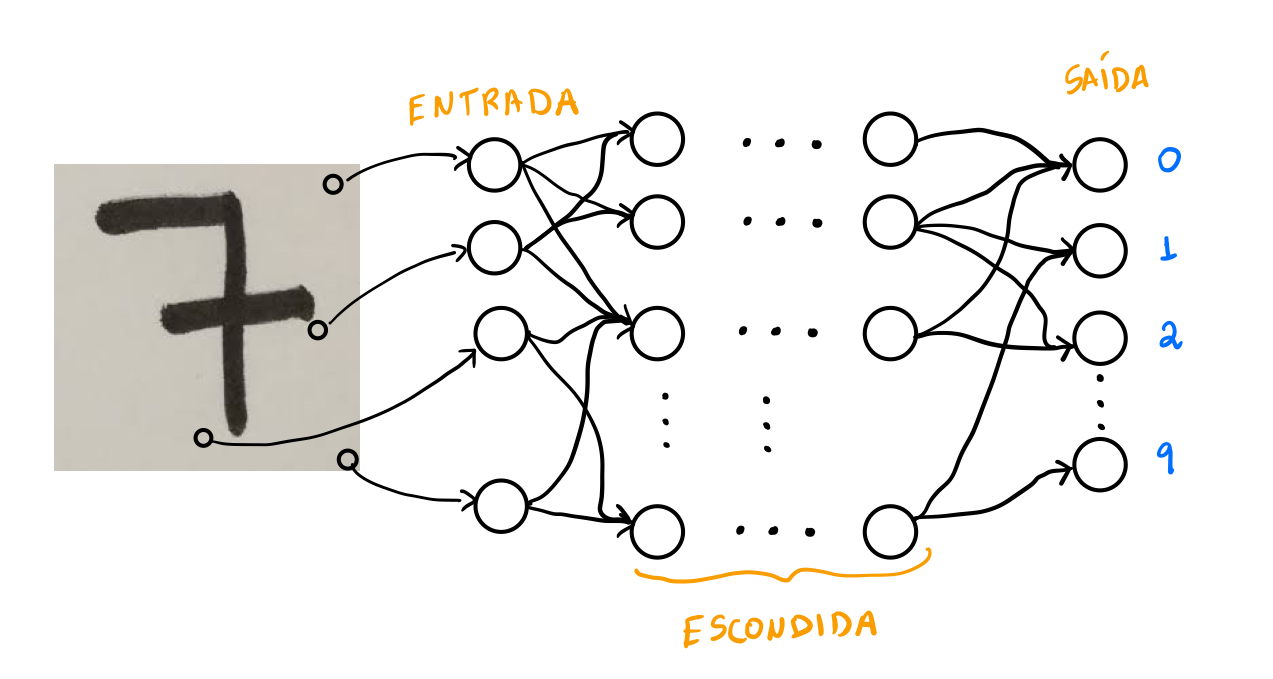
\includegraphics[scale=0.17]{./figs/CNN_Fig1.png}
\end{center}
}

\Sli{
\justifying De maneira geral, CNNs são compostas por dois módulos principais: (i) aprendizado de características e (ii) classificação. O aprendizado de características é realizado por meio de operações de convolução, agrupamento \emph{pooling} e aplicação da função de ativação. Já a etapa de classificação é composta, usualmente, por camadas do tipo \emph{fully connected} e uma camada de saída do tipo \emph{softmax}.

\begin{center}
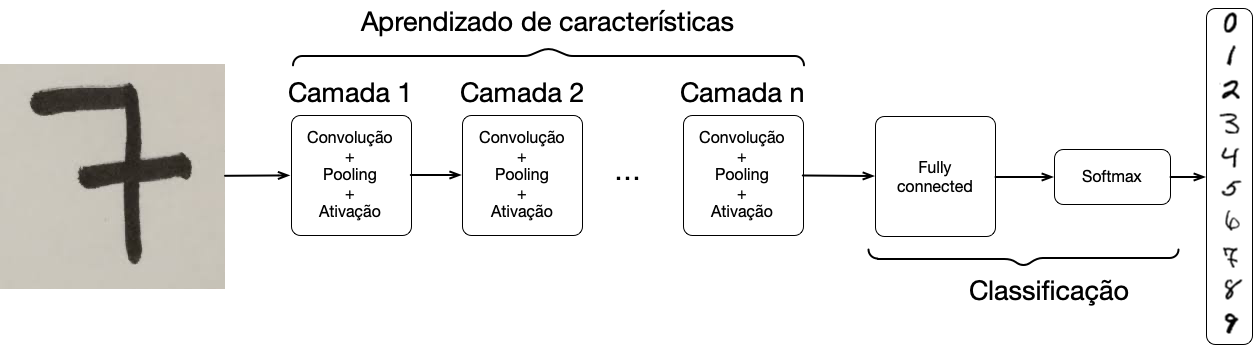
\includegraphics[scale=0.27]{./figs/CNN_Fig2.png}
\end{center}
}

\Sli{

\justifying Mas o que torna CNNs tão interessantes para diversas tarefas de classificação de padrões? O segredo está na etapa de \textbf{aprendizado de características}, em que informações importantes (textura, por exemplo) são aprendidas em diferentes níveis. O interessante é que essas redes são menos susceptíveis à problemas de rotação, translação e escala.\newline

\justifying Para entender o seu funcionamento, vamos estudar, primeiramente, o funcionamento de suas camadas de aprendizado de características e depois partir para as camadas de classificação. Como mencionado, cada camada da etapa de aprendizado é composta, basicamente, por operações de (ii) convolução, (iii) pooling e (iii) ativação.
}

\SliT{Aprendizado de Características}{
\secx{Convolução}\newline

\justifying A primeira operação que veremos é a de \textbf{convolução}, que é amplamente utilizada em tarefas de processamento de imagens e visão computacional, tais como filtragem de imagens (borramento e ruído) e detecção de bordas, por exemplo. Vejamos um exemplo.

\begin{center}
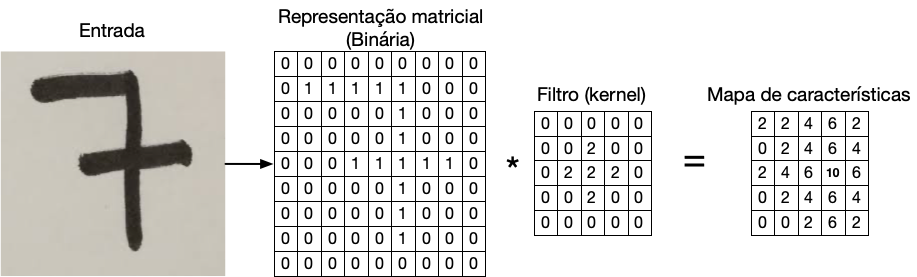
\includegraphics[scale=0.33]{./figs/CNN_Fig3.png}
\end{center}
}

\Sli{
\justifying A posição central da matriz de entrada $9\times9$ é substituída pelo valor obtido pela sua convolução com a máscara $5\times 5$ e o valor armazenado na matriz de saída $5\times 5$ (mapa de características). O procedimento é repetido até que toda a matriz de entrada tenha sido avaliada. Note que um trecho da matriz é descartado, por isso que a saída possui dimensões menores (podemos contornar isso com o \emph{zero padding} ou espelhamento da máscara).

\begin{minipage}{0.6\textwidth}
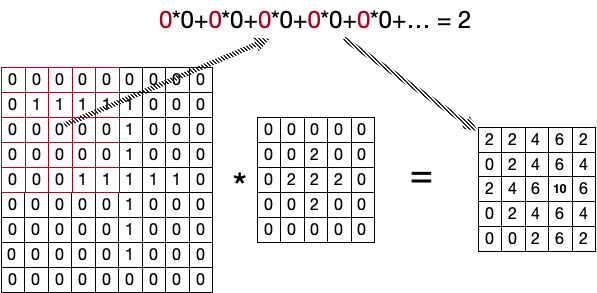
\includegraphics[scale=0.4]{./figs/CNN_Fig4.png}\end{minipage}%%% to prevent a space
\begin{minipage}{0.39\textwidth}
Como calcular o tamanho da saída? Suponha que as dimensões do dado de entrada e da máscara sejam, respectivamente, $m\times m$ e $n\times n$. O dado de saída terá a dimensão de $m-\lfloor n/2\rfloor\times m-\lfloor n/2\rfloor$.
\null
\par\xdef\tpd{\the\prevdepth}
\end{minipage}
}

\Sli{
Quais os hiperparâmetros envolvidos em uma operação de convolução? \textbf{Parâmetros $\times$ hiperparâmetros}.

\begin{itemize}
	\item Qual tipo de máscara (\emph{kernel}) iremos utilizar?
	\item Qual a melhor dimensão?
	\item Quantos filtros serão empregados?
	\item Qual o valor do \emph{stride}?
\end{itemize}
}

\Sli{
Dependendo do tipo de máscara utilizado, diferentes informações são obtidas na saída (\emph{feature maps}). Que tipo de informação de saída temos nos exemplos abaixo?\newline

\centerline{
\begin{tabular}{cc}
	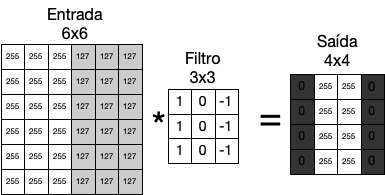
\includegraphics[scale=0.397]{./figs/CNN_Fig5.png} &\hspace{1cm}
	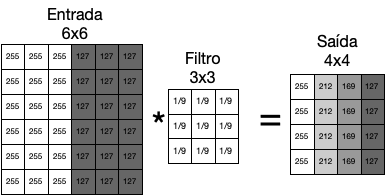
\includegraphics[scale=0.397]{./figs/CNN_Fig6.png} \\
	(a) Filtro passa-altas & (b) Filtro passa-baixas
\end{tabular}}
}

\Sli{
\justifying O que temos, na prática, são valores nas máscaras que podem ser interpretados como \textbf{pesos} que serão aprendidos pela CNN durante o seu processo de treinamento. Como calcular a quantidade desses parâmetros? Vejamos o exemplo abaixo (estamos assumindo \emph{padding}).

\begin{minipage}{0.51\textwidth}
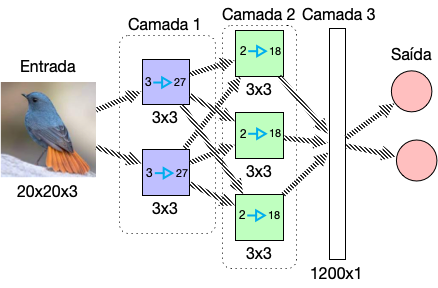
\includegraphics[scale=0.47]{./figs/CNN_Fig7.png}\end{minipage}%%% to prevent a space
\begin{minipage}{0.49\textwidth}
\begin{table}[]
\resizebox{\textwidth}{!}{%
\begin{tabular}{lccc}\hline
Camada            & Tipo                        & Entrada         & Saída                   \\\hline
Entrada           & Dado                     & 0               & 3                       \\
Intermediária 1 & Convolucional               & 3               & (27+27)+2 biases = 56        \\
Intermediária 2 & Convolucional               & 2               & 54+3 biases = 57        \\
Intermediária 3 & Flattened & -               & 20*20*3 = 1.200                       \\
Saída             & Densa                       & 1.200 & 1.200*2+2 biases = 2402 \\\hline
\end{tabular}%
}
\end{table}
{\scriptsize Quantidade de parâmetros a serem aprendidos: \textbf{2.515}.}
\null
\par\xdef\tpd{\the\prevdepth}
\end{minipage}
}

\Sli{
\justifying Qual o papel dos valores dos hiperparâmetros de uma CNN?

\begin{itemize}
	\item \justifying\underline{Tamanho do \emph{kernel}:} possui um papel muito importante em tarefas de classificação de imagens. \emph{Kernels} pequenos extraem uma quantidade maior de informações (\textbf{informações locais}) pois as reduções de tamanho entre as camadas são menores permitindo, assim, arquiteturas mais profundas. Por outro lado, \emph{kernels} maiores geram reduções mais rápidas no tamanho dos \emph{feature maps} e extraem informações mais \textbf{globais}.
	\item Valor de \emph{stride}: possui um impacto similar ao tamanho do \emph{kernel}, em que maiores valores proporcionam reduções mais rápidas dos \emph{feature maps}. Valores de \emph{stride} menores resultam em mais características aprendidas.
\end{itemize}
\justifying Dado que valores menores de \emph{stride} e de tamanho de \emph{kernels} proporcionam o aprendizado de mais características, por que não adotá-los sempre? \textbf{Isto requer bases de dados maiores.}
}

\Sli{
Resumindo, temos que tomar decisões sobre os seguintes itens acerca de uma camada de convolução:

\begin{enumerate}
	\item Tipo do \emph{padding}.
	\item Tamanho do \emph{kernel}.
	\item Valor de \emph{stride}.
\end{enumerate}
}

\Sli{
\secx{Ativação}\newline

\justifying CNNs, usualmente, são compostas por inúmeras camadas, não sendo interessante fazer uso de funções de ativação do tipo sigmoide ou tangente hiperbólica (problemas de saturação). Outra característica interessante das funções de ativação é sua característica de \textbf{não linearidade}, permitindo com que a rede aprenda funções de decisão não lineares.\newline

\justifying Umas das funções de ativação mais utilizadas é a ReLU (\emph{Rectified Linear Unit}) devido à sua simplicidade e alto grau de não linearidade. Sua formulação é dada como segue:

\begin{equation}
	\text{ReLU(x)} = \max\{0,x\}.
\end{equation}
}

\Sli{
Segue, abaixo, o gráfico da função \text{ReLU(x)}. Note que a função só retorna algo quando sua entrada possui valor maior do que $0$, ajudando no tempo de treinamento.

\begin{minipage}{0.49\textwidth}
\begin{center}
	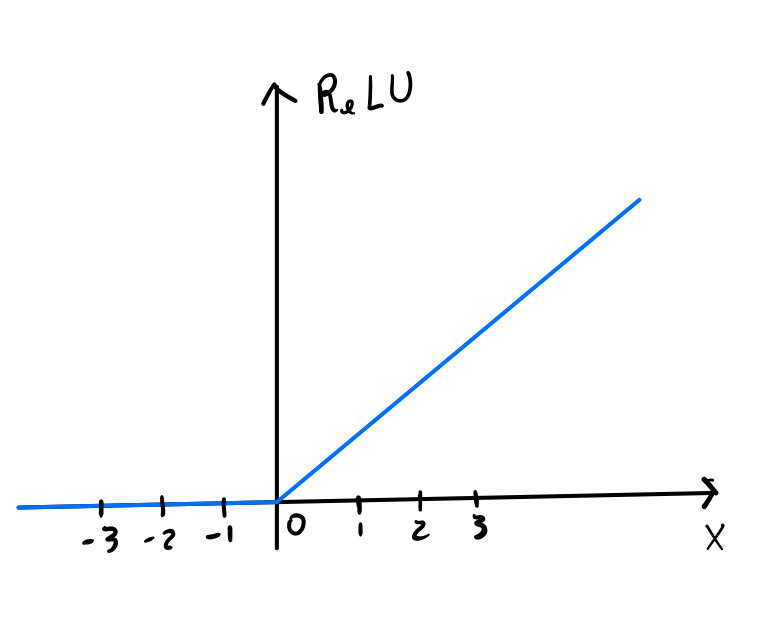
\includegraphics[scale=0.197]{./figs/CNN_Fig10.png}
\end{center}
\end{minipage}%%% to prevent a space
\begin{minipage}{0.5\textwidth}
A derivada da função \text{ReLU(x)} é dada como segue:

\begin{equation}
	\text{ReLU(x)}^\prime = 
	\begin{cases}
		0 \text{ caso $x \leq 0$} \\
		1 \text{ caso contrário.}
	\end{cases}
\end{equation}
\null
\par\xdef\tpd{\the\prevdepth}
\end{minipage}
}

\Sli{
\secx{Pooling}\newline

\justifying Existem diferentes tipos de operações de agrupamento ou \emph{pooling}, cujo objetivo principal é \textbf{diminuir a resolução} (\emph{downsampling}) dos \emph{feature maps} e adicionar \textbf{propriedades de invariância} à rede. A diminuição do tamanho dos \emph{feature maps} acarreta no decréscimo do número de parâmetros a serem aprendidos pela rede, permitindo um treinamento mais eficiente.\newline

\justifying Dentre os principais tipos de \emph{pooling}, podemos citar:

\begin{itemize}
	\item \emph{Max-Pooling}
	\item \emph{Average Pooling}
	\item \emph{Global Pooling}
\end{itemize}
}

\Sli{
\justifying Seguem algumas ilustrações para exemplificar o funcionamento dos tipos de \emph{pooling} mencionados anteriormente.\newline

\centerline{
\begin{tabular}{cc}
	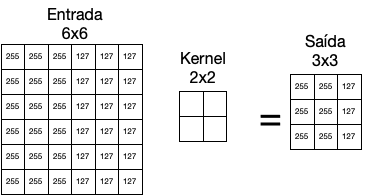
\includegraphics[scale=0.597]{./figs/CNN_Fig8.png} &\hspace{1cm}
	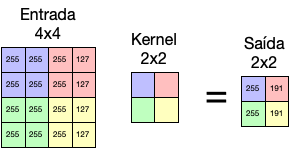
\includegraphics[scale=0.597]{./figs/CNN_Fig9.png} \\
	(a) Max-Pooling (stride = 2) & (b) Average Pooling (stride = 2)
\end{tabular}}
}

\Sli{
\justifying Já a técnica de \emph{global pooling} é mais radical no contexto de um \emph{downsampling}, pois reduz todo o \emph{feature map} em um único valor. Neste caso, podemos utilizar tanto \emph{max-pooling} quanto \emph{average pooling}.\newline

\justifying Geralmente, camadas de \emph{max-pooling} tendem a prover resultados melhores, pois é mais informativo utilizarmos o maior valor dentro de uma janela do que ``mascará-los"\ por meio do seu valor médio.
}

\Sli{
\secx{Flattening}\newline

\justifying Antes de enviar nossos dados que passaram pelas camadas de convolução, \emph{pooling} e ativação para as camadas do tipo \emph{fully connected} ou \emph{dense layers}, precisamos ``achatar"\ o \textbf{tensor} (dados). A operação nesta camada é bastante simples, dado que recebemos uma entrada com múltiplas dimensões (\emph{feature maps}) e a saída é um vetor unidimensional, como ilustrado abaixo.

\centerline{
\begin{tabular}{cc}
	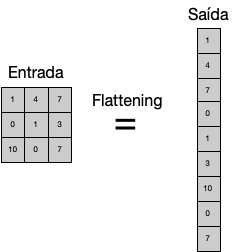
\includegraphics[scale=0.537]{./figs/CNN_Fig11.png} &\hspace{3cm}
	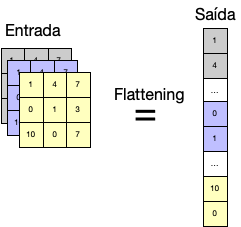
\includegraphics[scale=0.537]{./figs/CNN_Fig12.png} \\
\end{tabular}}
}

\Sli{
\secx{Fully Connected + Dropout}\newline

\justifying A parte final consiste em adotar camadas do tipo \emph{fully connected}, de maneira similar à uma Rede Neural MLP, com uma saída do tipo \emph{softmax} no final. Também é bastante comum adotarmos uma técnica de regularização conhecida por \emph{Dropout}, a qual ``remove"\ neurônios de maneira aleatória visando acelerar o processo de treinamento e prevenir \emph{overfitting}.

\begin{center}
	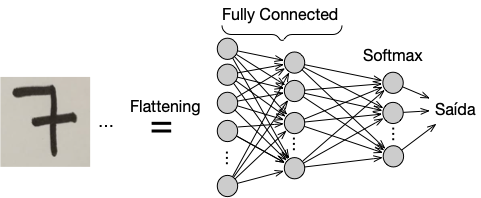
\includegraphics[scale=0.597]{./figs/CNN_Fig13.png}
\end{center}
}

\Sli{
\justifying A função \emph{softmax} $\sigma:\mathbb{R}^K\rightarrow [0,1]^K$ é uma generalização da função logística, em que $K$ corresponde ao número de classes.

\begin{minipage}{0.49\textwidth}
\begin{center}
	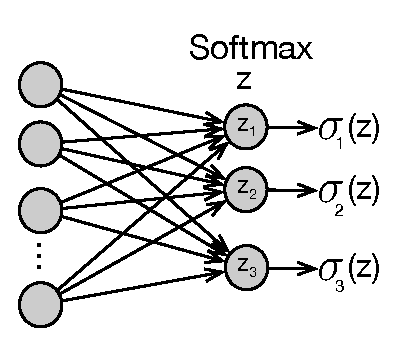
\includegraphics[scale=0.597]{./figs/CNN_Fig14.eps}
\end{center}
\end{minipage}%%% to prevent a space
\begin{minipage}{0.5\textwidth}
A sua formulação é dada como segue:
\begin{equation}
	\sigma_i(\mathbf{z}) = \frac{e^{z_i}}{\sum_{j=1}^Ke^{z_j}}.
\end{equation}
\null
\par\xdef\tpd{\the\prevdepth}
\end{minipage}

\justifying \textbf{Por que \emph{softmax} e não a função logística?} Usualmente, a função logística é aplicada em cada neurônio de saída sem considerarmos todos os outros. No caso, \emph{softmax} acaba resultando em uma probabilidade do neurônio de cada classe responder à um estímulo (dado) de entrada.
}

\SliT{Tipos de Operações de Convolução}{
\justifying Existem diferentes maneiras de executarmos a mesma tarefa de convolução, tais como:

\begin{itemize}
	\item Convolução Separada (\emph{Separable Convolution}) e 
	\item Convolução Dilatada (\emph{Dilated Convolution})
\end{itemize}

\justifying Usualmente, elas produzem o mesmo resultado no final, mas conseguem melhorar a eficiência do modelo em relação às convoluções tradicionais.
}

\Sli{
\secx{Convolução Separada}\newline

\justifying Consiste em ``quebrar"\ a convolução em \emph{kernels} com tamanhos menores. Existem dois tipos de convolução separada:

\begin{itemize}
	\item Convolução Separada Espacial (\emph{Spatially Separable Convolution}) e
	\item Convolução Separada em Profundidade (\emph{Depthwise Separable Convolution})
\end{itemize}

Vejamos, agora, cada um desses tipos.
}

\Sli{
\secxx{Convolução Separada Espacial}\newline

\justifying A convolução separada espacial, no caso 2D, consiste em aplicar duas convoluções 1D de maneira sequencial, de tal forma que o resultado final será o mesmo.\newline

\begin{minipage}{0.49\textwidth}
\begin{center}
	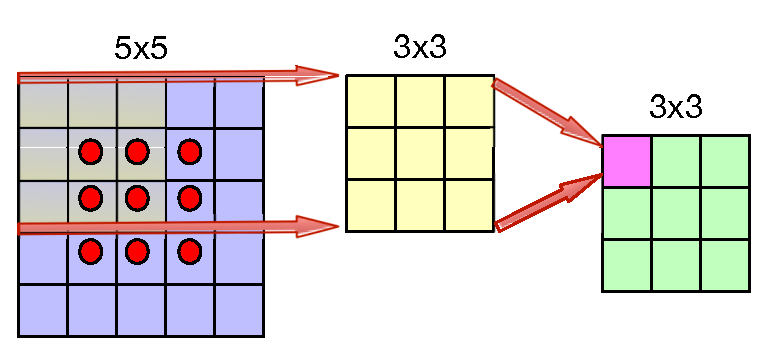
\includegraphics[scale=0.437]{./figs/CNN_Fig15.eps}
\end{center}
\end{minipage}%%% to prevent a space
\begin{minipage}{0.5\textwidth}
Cada um dos pontos vermelhos requer $3\times3=9$ operações de multiplicação. Desta forma, a convolução de todo o dado de entrada requer $9\times 9 = 81$ operações de multiplicação.
\null
\par\xdef\tpd{\the\prevdepth}
\end{minipage}
}

\Sli{
Vejamos, agora, o que acontece quando ``quebramos"\ uma convolução 2D em duas convoluções 1D.

\begin{center}
	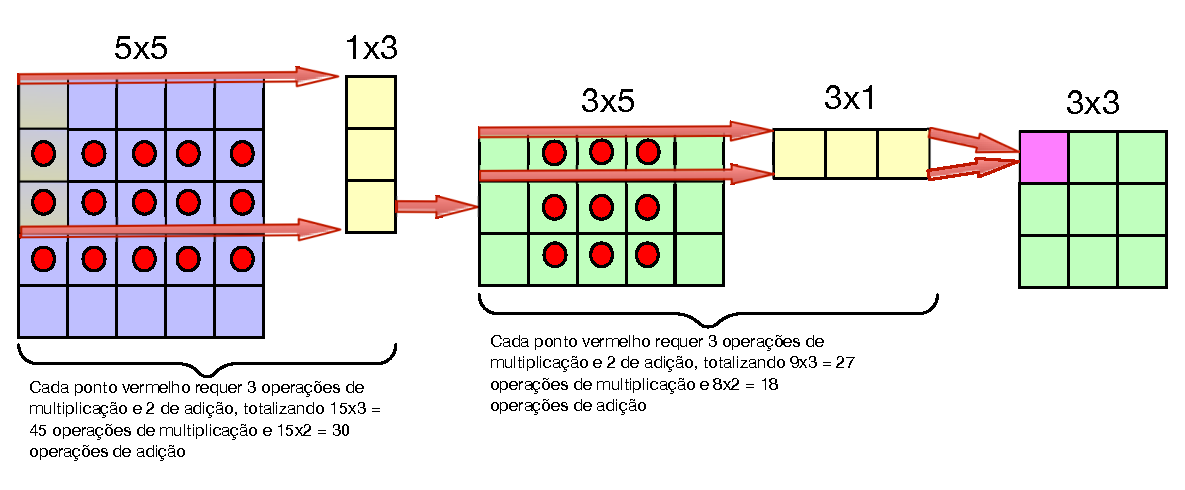
\includegraphics[scale=0.537]{./figs/CNN_Fig16.eps}
\end{center}

No total, teremos $45+27 = 72$ operações de multiplicação.
}

\Sli{
\secxx{Convolução Separada em Profundidade}\newline

\justifying A convolução separada em profundidade é aplicada em dados de entrada multidimensionais (imagens coloridas, por exemplo). A ideia consiste em aplicar a convolução em cada canal (dimensão) separadamente, e depois aplicar uma convolução do tipo pontual (\emph{pointwise convolution}). Primeiro, vamos entender como é feita a convolução em dados de entrada com múltiplas dimensões.

\begin{center}
	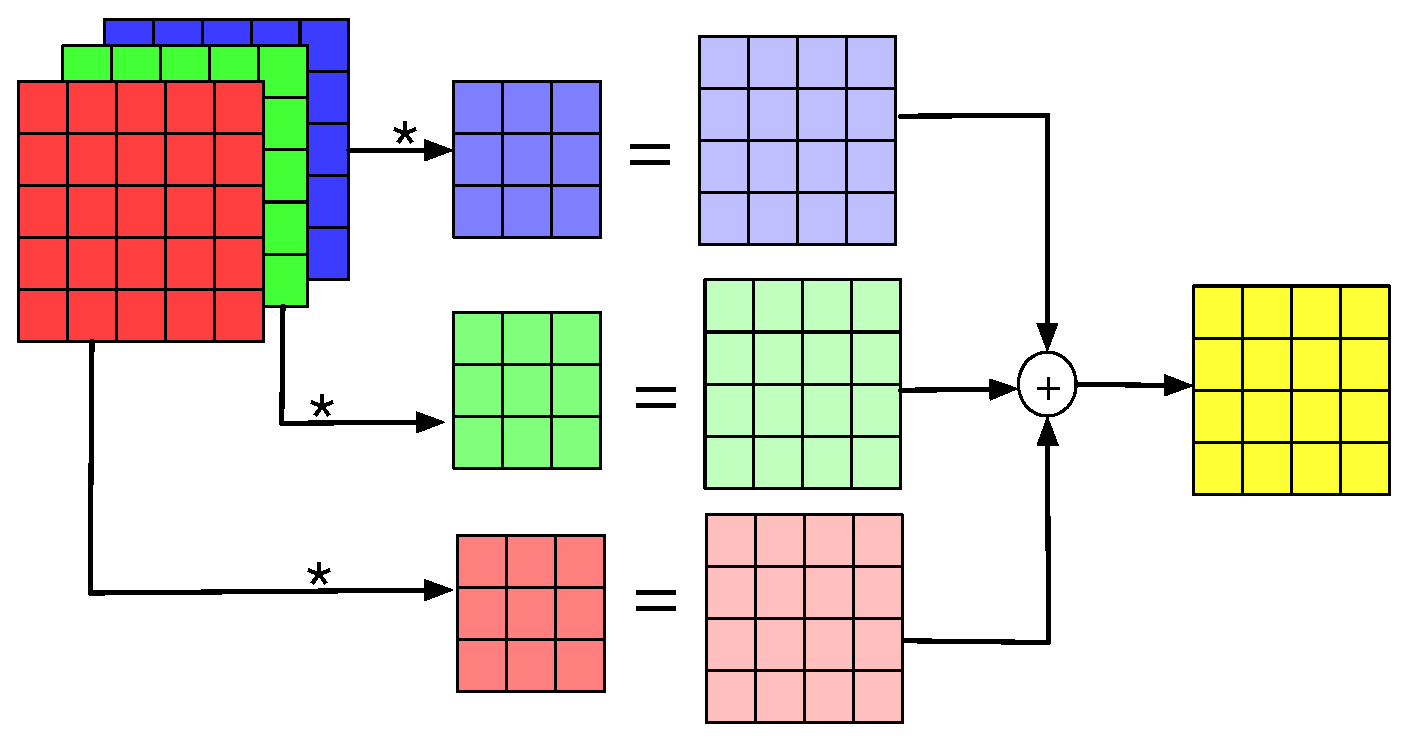
\includegraphics[scale=0.367]{./figs/CNN_Fig17.eps}
\end{center}
}

\Sli{
\justifying No caso de múltiplos filtros, a convolução com múltiplas dimensões pode ser representada da seguinte forma.

\begin{center}
	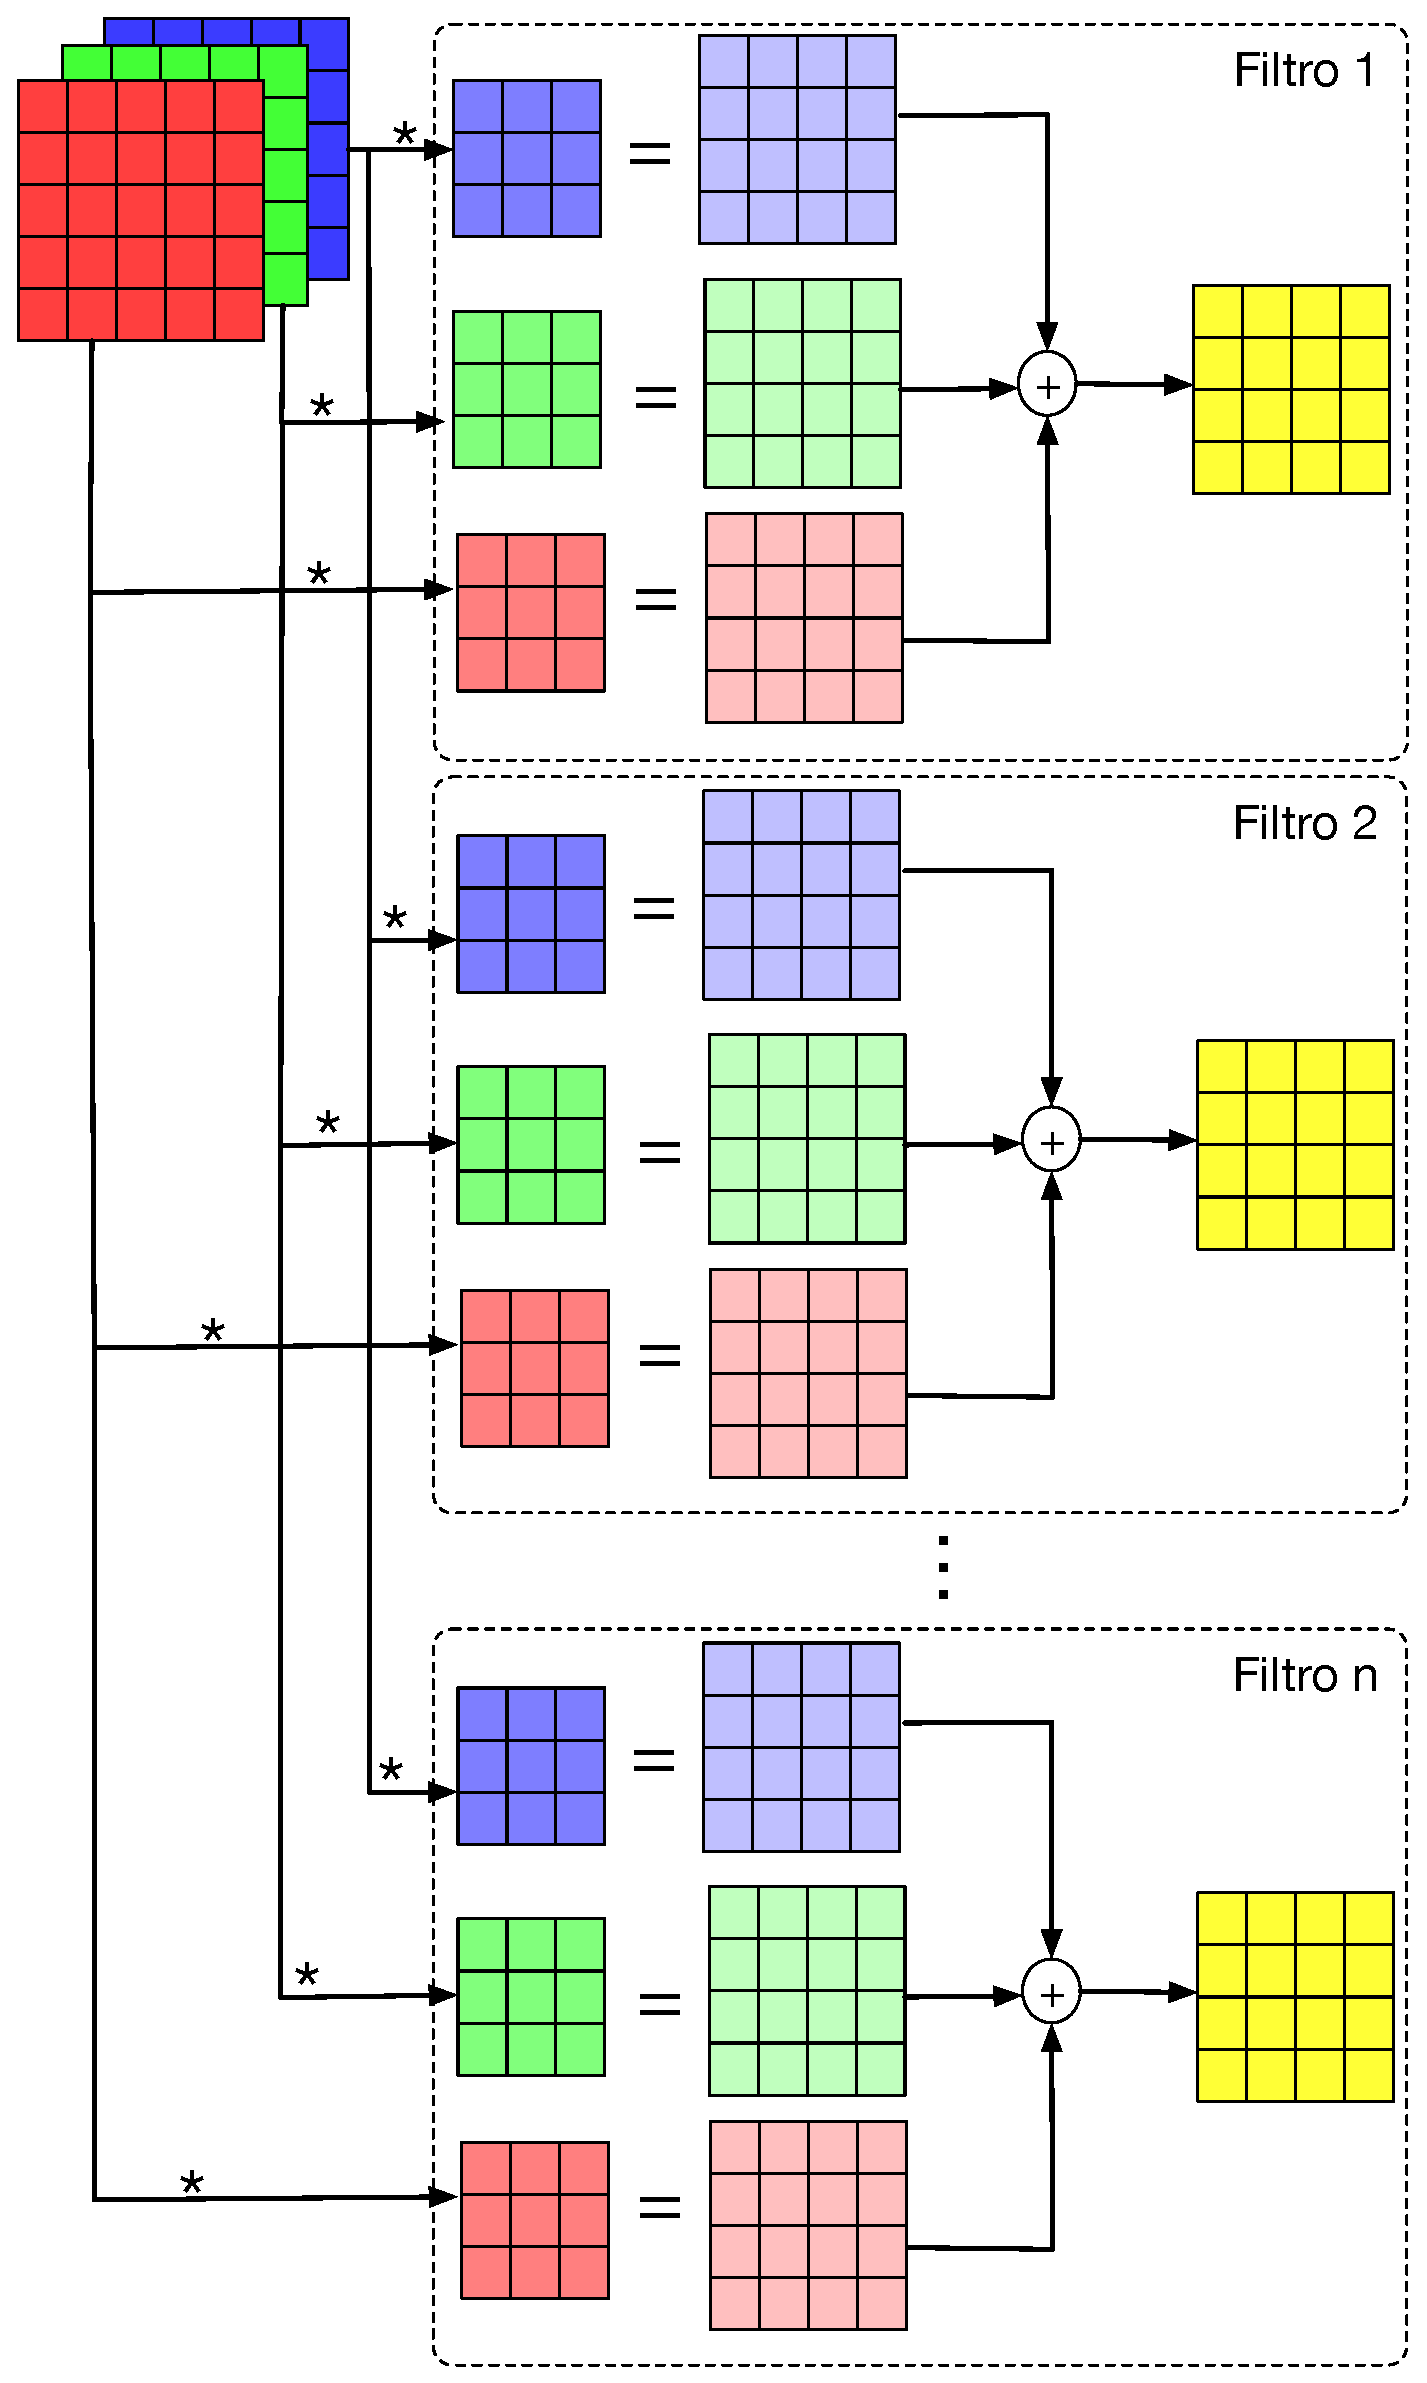
\includegraphics[scale=0.157]{./figs/CNN_Fig18.eps}
\end{center}
}

\Sli{
\justifying Vejamos, primeiramente, um exemplo de convolução com múltiplos filtros convencional.

\begin{center}
		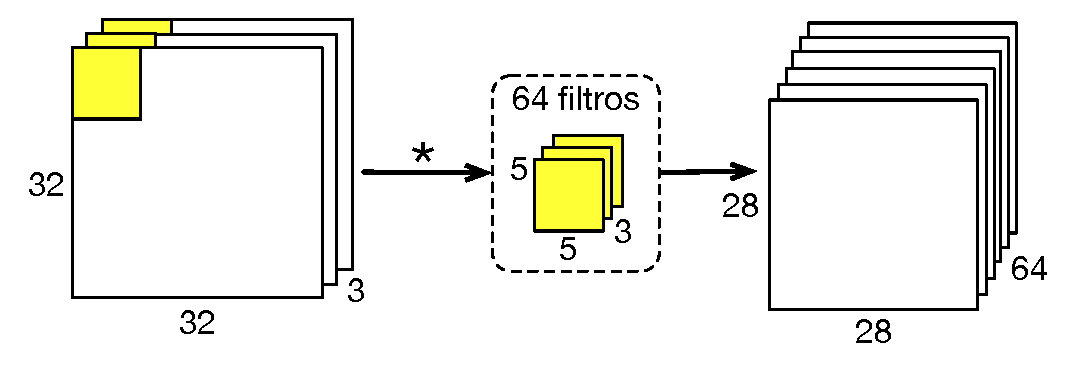
\includegraphics[scale=0.397]{./figs/CNN_Fig19.eps}
\end{center}

Aqui temos uma imagem de entrada $32\times32$ com $3$ canais (pode ser uma imagem colorida, por exemplo) cuja convolução será dada com uma máscara $5\times5\times3$. Serão aplicados $64$ filtros de tal forma que o \emph{feature map} de saída possui a dimensão $28\times28\times64$. \textbf{Assim, teremos uma quantidade de $5\times5\times3\times28\times28\times64=3.763.200$ operações de multiplicação.}
}

\Sli{
\justifying Vejamos, agora, um exemplo de convolução separada em profundidade.

\begin{center}
		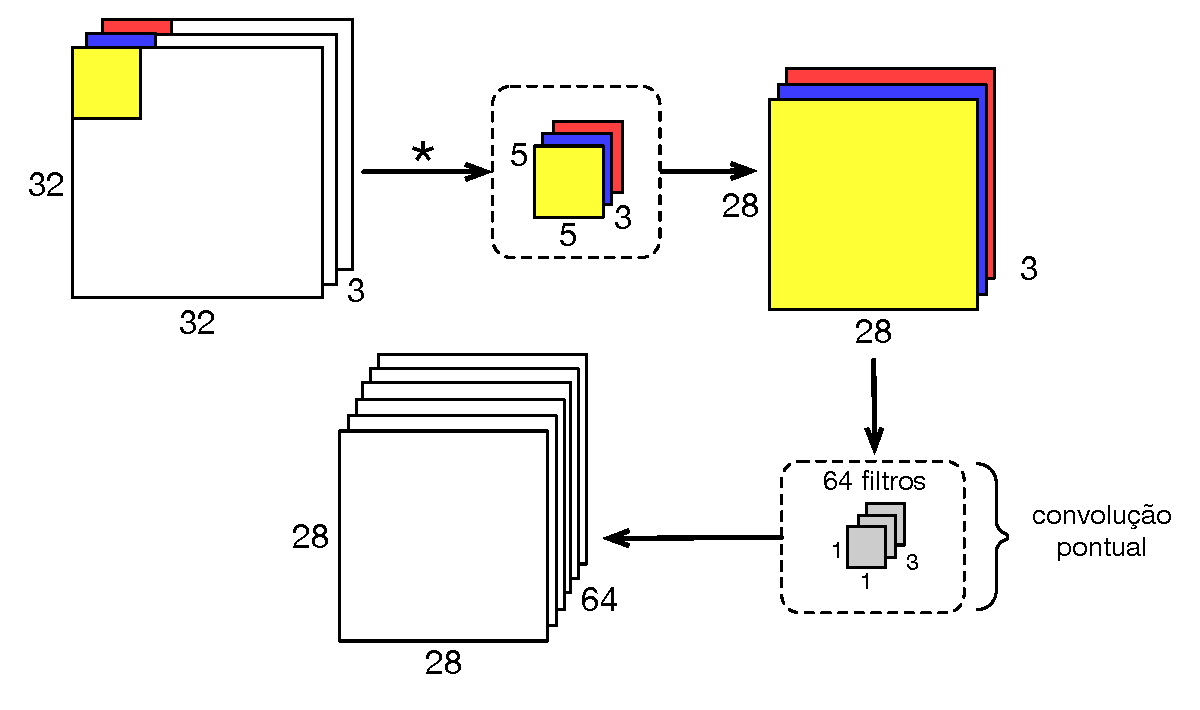
\includegraphics[scale=0.367]{./figs/CNN_Fig20.eps}
\end{center}

Nossa entrada $32\times32\times3$ passará por uma convolução com uma máscara $5\times5\times3$, gerando uma saída com dimensões $28\times28\times3$ e resultando em $5\times5\times3\times28\times28=58.800$ operações de multiplicação. Em seguida, os \emph{feature maps} passarão por uma convolução com uma máscara $1\times1\times3$ com $64$ filtros, resultando em $64\times1\times1\times3\times28\times28 = 150.528$ operações. \textbf{Ao final, teremos $58.800+150.528=290.328$ operações de multiplicação.}
}

\Sli{
\secx{Convolução Dilatada}\newline

\justifying 
}

\end{document}